%----------------------------1----------------------------------
\begin{frame}[t]{Motivación y Definición del Problema.}
  \begin{center}
    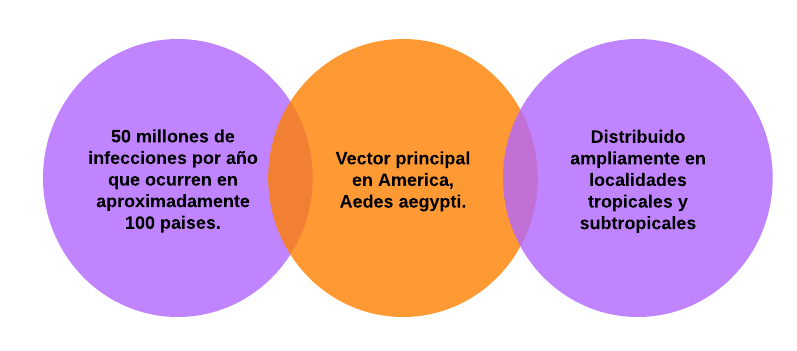
\includegraphics[width=10cm]{./graphics/dengue-intro.png}
  \end{center}
\end{frame}

%----------------------------2----------------------------------

\begin{frame}[t]{Motivación y Definición del Problema.\\\textit{Criaderos del Aedes aegypti.}}
\begin{center}
    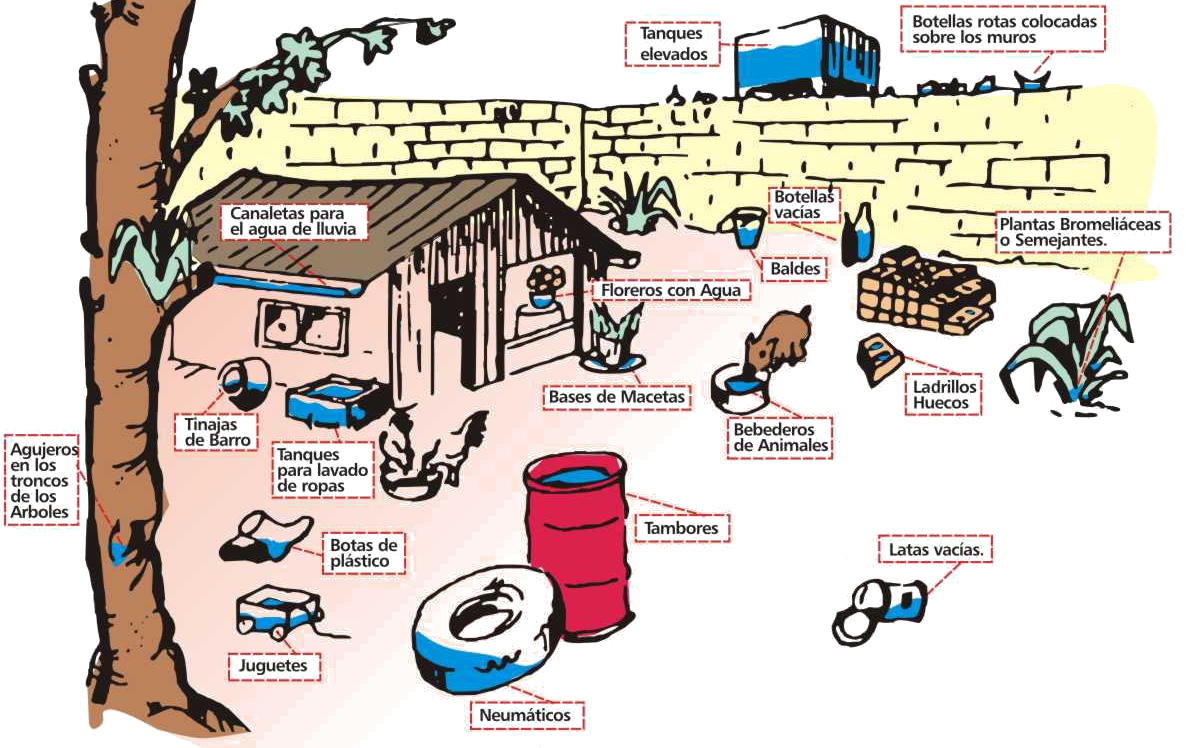
\includegraphics[width=9cm]{./graphics/criaderos.jpg}
    \end{center}
\end{frame}

%----------------------------3----------------------------------


%----------------------------4----------------------------------

\begin{frame}[t]{Motivación y Definición del Problema.\\\textit{Dengue en Paraguay.}}
  \begin{center}
    \begin{itemize}
    \item El Paraguay desde el año 2009 es considerado un país endémico.

    \item El clima, subtropical, favorece la aparición y desarrollo del dengue.

    \item Se realizan actividades de monitoreo del comportamiento el vector mediante técnicas tradicionales de vigilancia.

    \item Se utilizan técnicas de control vectorial, como fumigación, para la disminución de las poblaciones de mosquitos.

    \item En las últimas décadas se han observado un crecimiento considerable de las notificaciones de posibles casos de dengue, algunas con derivaciones fatales.
    \end{itemize}
  \end{center}
\end{frame}

%----------------------------5----------------------------------

\begin{frame}[t]{Motivación y Definición del Problema.\\\textit{Dengue en Paraguay.}}
  \begin{center}
  \begin{table}
      \begin{minipage}{\textwidth}
          \begin{center}
          \caption{Histórico de casos de dengue notificados, confirmados y con derivación fatal en Paraguay.}
          \begin{tabular}{l c c r r}
              \hline
              Año & Periodo (inicio / fin) & Notificados & Confirmados & Muertes\\
              \hline
              \hline
              2014 & 29-12-13 / 31-05-14 & 10.541 & 1.052 & 2\\
              2013 & 30-12-12 / 21-12-13 & 153.793 & 131.306 & 70\\
              2012 & 01-01-12 / 22-12-12 & 37.815 & 30.588 & 11\\
              2011 & 03-01-11 / 29-12-11 & 53.397 & 42.264 & 62\\
              2010 & 11-10-09 / 25-12-10 & 21.951 & 13.760 & --$^a$
          \end{tabular}
          \footnotetext[1]{No se encontraron datos sobre muertes en el periodo.}
          \end{center}
      \end{minipage}
  \end{table}
  \end{center}
\end{frame}

%----------------------------6----------------------------------

\begin{frame}[c]{Motivación y Definición del Problema.\\\textit{Vigilancia Entomológica en Paraguay.}}

    \begin{itemize}
      \item La Vigilancia Entomológica es un proceso orientado al levantamiento de información sobre la distribución del Aedes aegypti y la medición relativa de su población.

      \item Para estimar la densidad del vector, la OMS ha recomendado los siguientes indicadores entomológicos : Índice de Casa, Índice de Recipiente e Índice de Breteau.

      \item Sólo son recomendados para detectar la calidad de las acciones realizadas por el personal de control larvario.

      \item Las autoriadades sanitarias del Paraguay utilizan estos índices para estimar la densidad poblacionál del vector.

    \end{itemize}
\end{frame}

\begin{frame}[c]{Motivación y Definición del Problema.\\\textit{Vigilancia Entomológica en Paraguay.}}
\begin{itemize}
      \item Actualmente son considerados, por la OMS, como una pobre indicación de la producción de mosquitos adultos.

      \item No reflejan la asociación que existe entre las densidades de mosquitos y los tipos de recipientes.

      \item Proporcionan poca o nula información de aquellas viviendas en las que existe un mayor riesgo de presencia de mosquitos.

      \item Existen numerosos métodos e indicadores más prácticos, eficientes y económicos, como larvitrampas y ovitrampas.

    \end{itemize}
\end{frame}

%----------------------------7----------------------------------

\begin{frame}[t]{Motivación y Definición del Problema.\\\textit{Larvitrampas.}}
  \begin{center}
    \begin{columns}[c]
        \begin{column}[c]{3cm}
          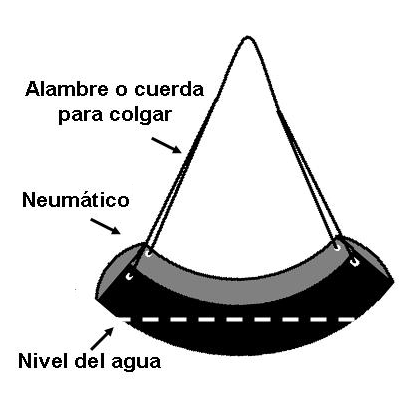
\includegraphics[width=\textwidth]{../book/anexos/graphics/disenho-1.png}

          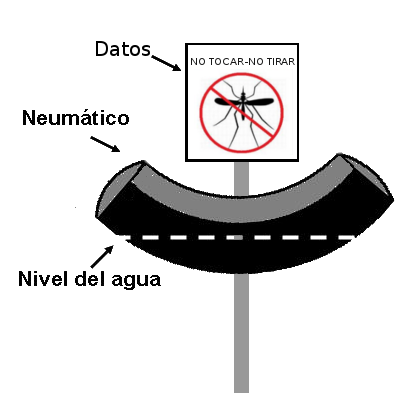
\includegraphics[width=\textwidth]{../book/anexos/graphics/disenho-2.png}
        \end{column}
        \begin{column}[c]{7cm}
          \begin{itemize}
            \item Criadero artificial y controlado.
            \item Se basan en la detección del vector en su etapa larval.
            \item Brinda información sobre los patrones de actividad espacial y estacional de ovipostura.
            \item Permiten reconocer las condiciones climáticas favorables para la eclosión y desarrollo larvario.
            \item Materiales reciclados como materia prima.
          \end{itemize}
        \end{column}
      \end{columns}
  \end{center}
\end{frame}

\begin{frame}[t]{Motivación y Definición del Problema.\\\textit{Larvitrampas.}}
  \begin{center}
    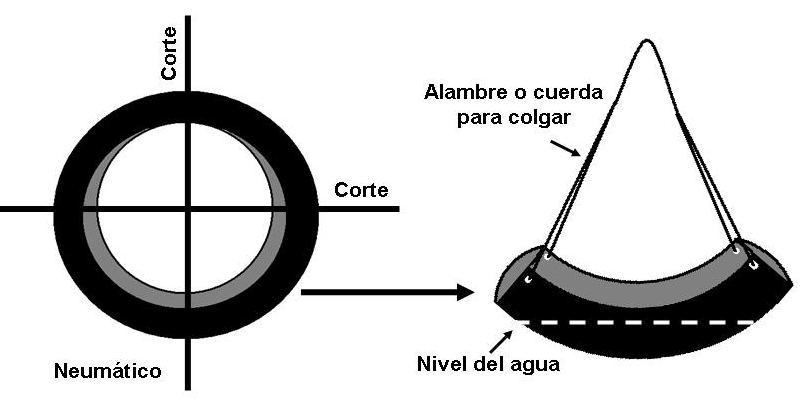
\includegraphics[width=9cm]{../book/anexos/graphics/construccion-larvitrampa.png}
  \end{center}
\end{frame}

%----------------------------6----------------------------------
\begin{frame}[t]{Motivación y Definición del Problema.
\\\textit{La problemática del dengue en Paraguay.}}
  \begin{itemize}

    \item Las autoridades sanitarias del Paraguay no cuentan con datos computables, geográficamente, referentes al dengue, que permitan realizar análisis estadísticos y espaciales.

    \item Se deben diseñar y desarrollar herramientas para la recolección de la información, para su posterior análisis.

    \item Se deben optar por nuevas metodologías que permitan generar información para el análisis sin la necesidad de grandes requerimientos.

    \item Las larvitrampas y ovitrampas permiten generar información regionalizada sobre el estado y la distribución de la población del vector.

  \end{itemize}
\end{frame}

